\section{Implementation}
\label{chap:MediaProject}

This part forms the core of the work. Here I present the design and development of \textbf{\ns}, an \glsit{opensource} \gls{vn} engine entirely driven by text files in \gls{json} format. The author writes their story in a \gls{json} file that conforms to the defined \gls{schema}, then puts the project online either by compiling the \gls{reactjs} application into static files via \texttt{npm run build}, or through a continuous integration platform such as Vercel\footnote{\textbf{Vercel}: cloud deployment platform specialised in static web applications and \gls{js} frameworks. It automates building and deployment on every change to the source repository. \parencite{noauthor_vercel_nodate}} or GitHub Pages\footnote{\textbf{GitHub Pages}: static hosting service built into GitHub, allowing a repository's content to be automatically published as a website accessible via a public URL, with no server configuration. \parencite{noauthor_documentation_nodate}}. The final \gls{vn} thus remains accessible from any modern web browser, with no installation required on the player's side. The project's source code is publicly available on GitHub at the following address: \nsrepo.

The development followed an iterative logic: each iteration corresponded to a set of features that were implemented, tested, and evaluated before moving on to the next step.


\subsection{Scope Evolution: From Library to Application}

Initially, I had planned to develop \nsits as a \gls{reactjs} \gls{librairie} publishable on \gls{npm}, integrable by a third-party developer through a simple install command. The idea was to distribute the engine as a reusable component, independent of any host application.

To learn how to implement this architecture, two resources were consulted: a 2024 YouTube playlist by Imran Hussain (username \textit{Imran Codes}), titled \textit{Building a React Component Library: A Senior Developer's Guide}\parencite{imran_codes_1_2024} (targeting \gls{reactjs} 16), and a text article by Alex Eagleson published on dev.to in November 2021 and updated in December 2022 \parencite{noauthor_how_2021} (targeting \gls{reactjs} 17 and rollup\footnote{\textbf{Rollup}: \gls{js} bundling tool specialised in building distributable \gls{librairie}s. In \textit{\gls{librairie} mode}, it compiles the source code into one or more optimised files, together with \gls{ts} type definitions, ready to be published as an \gls{npm} \glsit{package}. \parencite{noauthor_introduction_nodate}} V2). Both resources relied on the same approach: configuring rollup in \gls{librairie} mode via a \texttt{rollup.config.js} file, combining the \texttt{@rollup/plugin-typescript}, \texttt{@rollup/plugin-commonjs}, and \texttt{rollup-plugin-dts} \glspl{plugin}.

\clearpage

In both cases, the \glsit{build} command (\texttt{npm run build}) failed. The errors encountered stemmed from the rollup configuration, whose requirements changed across successive versions of the tool. Eagleson's article itself flags this problem: a note embedded in the text indicates that some tools have been updated and that the instructions as written no longer work. \parencite{noauthor_how_2021} The comments on both resources, also roughly a year old, offered partial fixes that did not resolve the problem in the context of \gls{reactjs} 19 and current versions of rollup.

No more recent resource based on a configuration adapted to \gls{reactjs} 19 could be identified; the available tutorials all used the same configuration approach, which has become incompatible with current versions of the tooling. It cannot be ruled out that some of the errors encountered resulted from a misinterpretation of the configuration steps on my part; this possibility cannot be excluded.

Faced with these obstacles and the project's time constraints, the decision was made to redirect the architecture toward a standalone \gls{reactjs} application. This more directly manageable approach achieves the project's main objective: making \gls{vn} creation accessible via the web, without requiring the distribution of an \gls{npm} \glsit{package}.

\clearpage


\subsubsection{Technical Stack and Tools}

The development of \nsits relies on the technologies and tools listed in Table \ref{tab:stack}.

\begin{table}[H]
    \centering
    \caption{Technical stack and tools used}
    \renewcommand{\arraystretch}{1.5}
    \begin{tabular}{p{4cm} p{9cm}}
        \hline
        \textbf{Tool / Technology} & \textbf{Role in the project} \\
        \hline
        \gls{reactjs} & \Gls{librairie} \gls{js} used to render the engine in the browser. \\
        \addlinespace
        \gls{vite} & \Glsit{build} tool and development server, enabling fast hot-reloading during development. \\
        \addlinespace
        \gls{ts} & Typed superset of \gls{js}, used to strengthen code robustness and make it easier to catch errors before runtime. \\
        \addlinespace
        \gls{json} & Format used to describe narrative content, serving as the engine's single source of truth \\
        \addlinespace
        GitHub & Source code hosting and version control platform, via \gls{git}. \\
        \hline
    \end{tabular}
    \label{tab:stack}
\end{table}

\clearpage


\subsubsubsection{React.js Optimisation Mechanisms} \label{sec:optim_react}

\gls{reactjs} offers several mechanisms for reducing the number of unnecessary \glspl{rendu} and improving an application's performance. Three of them were used in this project \parencite{noauthor_reference_nodate}:

\texttt{React.memo} is a function that \glslink{override}{short-circuits} a component's \gls{rendu} if its \texttt{props}\footnote{\textbf{Props} (\textit{properties}): in \gls{reactjs}, a read-only object passed to a component by its parent component to configure its display or behaviour. \parencite{noauthor_reference_nodate}} have not changed since the previous \gls{rendu}. Without this mechanism, any state change in a parent component triggers the recomputation of all of its child components, whether or not they are affected by the change.

\texttt{useMemo} is a \glsit{hook} in \gls{reactjs} that caches the result of an expensive computation between two \glspl{rendu}. The computation is only rerun if one of its declared dependencies has changed, avoiding unnecessary recomputation on every \gls{rendu}.

\texttt{useRef} is a \glsit{hook} that persists a value across \glspl{rendu} without triggering a \glslink{rendu}{re-render} when it changes. It is used to store references to \acrshort{dom} elements or internal values whose change should not trigger an interface update.


\subsubsection{Development Method}

Development followed an iterative process based on the \glsit{pdca} cycle (\textit{Plan, Do, Check, Act}), as defined in the methodology presented in Section \ref{sec:PDCA}. Each iteration corresponds to a full cycle: planning the features to implement, development, evaluation through functional tests, then deciding on the adjustments to make for the next iteration.

This model was chosen for its ability to continuously incorporate evaluation feedback, without needing to redefine the entire scope at each step.

\clearpage


\subsection{Constraints and Limitations}

\subsubsection{Deployment Constraint}

Unlike traditional game engines that compile the project into a native executable, \nsits relies on web technologies. To create a \gls{vn} with this engine, the author must download the project, then write their story in a \gls{json} file following the defined \gls{schema}. The result can then be put online in two ways:

\begin{itemize}
    \item By compiling the \gls{reactjs} application into static files via the \texttt{npm run build} command, then hosting those files on any web server or static host.
    \item By connecting the repository to a continuous integration platform such as Vercel or GitHub Pages, which automatically handles building and deployment on every change to the project.
\end{itemize}

In both cases, the final \gls{vn} is accessible from any modern web browser, with no installation required on the player's side; see Figure \ref{fig:deploiement-flux}.

\begin{figure}[H]
    \centering
    \begin{tikzpicture}[
        node distance = 0.3cm and 0.3cm,
        every node/.style = {font=\scriptsize, align=center},
        box/.style = {
            rectangle, rounded corners=3pt,
            draw=clrBorder, line width=0.7pt,
            minimum width=2.1cm, minimum height=0.7cm,
            inner sep=3pt
        },
        auteur/.style = {box, fill=clrAuteur},
        build/.style  = {box, fill=clrBuild},
        cloud/.style  = {box, fill=clrCloud},
        player/.style = {box, fill=clrPlayer},
        alt/.style    = {box, fill=clrAlt},
        arrow/.style  = {-{Latex[length=4pt,width=3pt]},
                         line width=0.7pt, color=clrArrow},
        lbl/.style    = {font=\tiny\itshape, color=clrNote},
    ]

%% ── Row 1: Preparation (Author) ─────────────────────────────────────────
\node[auteur] at (0,0) (dl)
    {Getting the project\\
     \tiny{\texttt{git clone} / ZIP}};

\node[auteur, right=of dl]      (content)
    {Writing JSON + assets\\
     \tiny{story, characters, media}};

\node[auteur, right=of content] (config)
    {Configure \texttt{App.tsx}\\
     \tiny{\texttt{scriptFile=...}}};

\node[auteur, right=of config]  (push)
    {Commit \& push\\
     \tiny{to GitHub}};

\draw[arrow] (dl)      -- (content);
\draw[arrow] (content) -- (config);
\draw[arrow] (config)  -- (push);

%% ── Row 2, left: CI/CD path ───────────────────────────────────────────
\node[cloud] at (-0.8,-1.8) (cicd)
    {Push detected\\
     \tiny{Vercel / GitHub Pages}};

\node[build, right=of cicd]     (buildci)
    {Build\\
     \tiny{\texttt{tsc \&\& vite} $\to$ \texttt{dist/}}};

\node[cloud, right=of buildci]  (deployci)
    {Auto deployment\\
     \tiny{public URL}};

\draw[arrow] (cicd)    -- (buildci);
\draw[arrow] (buildci) -- (deployci);

%% ── Row 2, right: Manual path ─────────────────────────────────────────
\node[build] at (7.2,-1.8) (buildman)
    {Local build\\
     \tiny{\texttt{npm run build} $\to$ \texttt{dist/}}};

\node[alt, right=of buildman]   (upload)
    {Manual upload\\
     \tiny{static host}};

\node[alt, right=of upload]     (deployman)
    {Deployment\\
     \tiny{public URL}};

\draw[arrow] (buildman) -- (upload);
\draw[arrow] (upload)   -- (deployman);

%% ── Arrows push → paths ────────────────────────────────────────────────────
\draw[arrow] (push.south) -- ++(0, -0.4cm) -| (buildman.north);
\draw[arrow] (push.south) -- ++(0,-0.4cm) -| (cicd.north);

%% ── Row 3: Execution (Player) ───────────────────────────────────────────
\node[player] at (6.4,-3.6) (browser)
    {Browser\\
     \tiny{loading the URL}};

\node[player, right=of browser] (zodwk)
    {Zod validation\\
     \tiny{+ Web Worker}};

\node[player, right=of zodwk]   (vn)
    {VN rendering\\
     \tiny{\texttt{VNPlayer} component}};

\draw[arrow] (deployci)  |- (browser.west);
\draw[arrow] (deployman) |- (4.4cm, -2.5cm) |- (browser.west);
\draw[arrow] (browser) -- (zodwk);
\draw[arrow] (zodwk)   -- (vn);

%% ── Grouping boxes ───────────────────────────────────────────────────
\begin{scope}[on background layer]
  \node[draw=clrBorder, dotted, rounded corners=5pt, fill=clrAuteur!20,
        fit=(dl)(content)(config)(push), inner sep=6pt,
        label={[font=\tiny\bfseries, text=clrBorder]above:Preparation (Author)}
       ] {};

  \node[draw=clrBorder, dotted, rounded corners=5pt, fill=clrCloud!20,
        fit=(cicd)(buildci)(deployci), inner sep=6pt,
        label={[font=\tiny\bfseries, text=clrBorder, yshift=-2pt]above:CI/CD path}
       ] {};

  \node[draw=clrBorder, dotted, rounded corners=5pt, fill=clrAlt!20,
        fit=(buildman)(upload)(deployman), inner sep=6pt,
        label={[font=\tiny\bfseries, text=clrBorder, yshift=-2pt]above:Manual path}
       ] {};

  \node[draw=clrBorder, dotted, rounded corners=5pt, fill=clrPlayer!20,
        fit=(browser)(zodwk)(vn), inner sep=6pt,
        label={[font=\tiny\bfseries, text=clrBorder, yshift=-2pt]above:Execution (Player)}
       ] {};
\end{scope}

    \end{tikzpicture}
    \caption{Deployment flow of \nsit, from local configuration to execution in the browser (Author 2026)}
    \label{fig:deploiement-flux}
\end{figure}

\clearpage

\subsubsection{Format Constraint}

A fundamental constraint of this project is making the narrative content readable and interpretable both by a human and by a machine. The \gls{json} format was chosen to meet this requirement: its key/value model is sufficiently structured to be parsed deterministically by the \gls{parseur}, while remaining accessible to a non-developer author willing to follow a documented \gls{schema}.

However, this constraint carries an inherent limitation: the absence of semantic interpretation of natural language means the author must strictly follow the defined \gls{syntaxe}. A structural error in the \gls{json} file can block the engine's execution. Handling these errors and giving the author clear feedback are therefore a robustness goal to be addressed across the iterations.


\subsubsection{Scope Constraint}

For time reasons, the engine's functional scope is limited to the core \gls{vn} mechanics, as defined in Table \ref{tab:objectifs_moscow}. Other features, such as background music, character images, or a save system, are identified as desirable, but are not part of this work's primary objectives.


\subsection{Development Stages}

The development of \nsits took place over three successive iterations, each following the \glsit{pdca} cycle defined in Section \ref{sec:PDCA}. The objectives of each iteration were defined beforehand according to the \glsit{moscow} prioritisation set out in Table \ref{tab:objectifs_moscow}, and adjusted based on the results observed at the end of each cycle.


\subsubsection{First Iteration: The Basics of a VN}


\subsubsubsection{Plan}

The objective of this first iteration was to implement the engine's core mechanics: progressive text display (typewriter effect), scene navigation, and dialogue choice handling. These three features correspond to the \textit{Must} requirements in Table \ref{tab:objectifs_moscow}. It also involved defining the structure of the \gls{json} \gls{schema} used as the content source, i.e. the node types the engine would need to be able to interpret: dialogue, choice, scenes, and characters.


\subsubsubsection{Do}

I started by creating the project. To do so, I needed to choose a language, a \glsit{framework}, and a structure. For the language, I chose \gls{ts}, to benefit from static typing that provides safety as early as the development phase, before runtime even begins. As for the \glsit{framework}, I hesitated with Next.js\footnote{\textbf{Next.js}: server-rendering-oriented \gls{reactjs} \glsit{framework}, developed by Vercel \parencite{noauthor_nextjs_nodate}}, but it would have been overkill for this project: \nsits requires no server-side processing (\textit{\glsit{backend}}), with everything computed in the \glsit{frontend}. I therefore chose \gls{reactjs}, a \gls{js} \gls{librairie} I was already familiar with and which is perfectly suited to building this component-based project, allowing each part of the code to be kept separate.

Even before starting to build a single component, I began thinking about the structure I wanted to use for the \gls{json} file that would hold the story. I wanted something customisable, to leave as much freedom as possible to people wanting to use this project. To achieve this, I had to separate out several elements, illustrated in Table \ref{tab:obj_json_schema}.

\begin{table}[H]
    \centering
    \caption{Separation of the JSON file's main elements}
    \renewcommand{\arraystretch}{1.5}
    \begin{tabular}{p{4cm} p{9cm}}
        \hline
        \textbf{Object} & \textbf{Description} \\
        \hline
        Settings & Definitions of the application's global default values: customisation of the title screen, the credits page, and display behaviour. These values can be \glslink{override}{overridden} locally at the dialogue level. \\
        \addlinespace
        Characters & The declaration of characters, so that all characters and their information live in a single place. \\
        \addlinespace
        The story & All the elements used to tell the story. \\
        \hline
    \end{tabular}
    \label{tab:obj_json_schema}
\end{table}

Why these choices? Why not put the characters inside the story? There are several answers to these questions. To begin with, it gives a simple, readable structure: everything is separated according to clear, distinct purposes: what helps the author (settings), what will be used repeatedly (characters), and the narrative itself. Characters, like variables, are likely to appear across many scenes. Centralising them thus avoids any repetition in the file.

\clearpage

Code listing \ref{lst:json_example} shows this separation in a short example.

\begin{listing}[H]
\begin{minted}{json}
{
    "settings": {
        "startingScene": "start",
        "textSpeed": 45
    },
    "characters": {
        "Alice": {
            "name": "Alice",
            "fullName": "Alice Wonderland",
            "color": "#e07ae0"
        }
    },
    "story": {
        "start": {
            "background": "bg.png",
            "dialogues": [
                {
                    "name": "Alice",
                    "text": "Hello, world."
                },
                {
                    "name": "Alice",
                    "text": "Where shall we go?",
                    "options": [
                        { "text": "The library", "next": "library" },
                        { "text": "The park", "next": "park" }
                    ]
                }
            ]
        }
    }
}
\end{minted}
\caption{Example JSON file structure (Author 2026)}
\label{lst:json_example}
\end{listing}

\clearpage

As the iterations progressed, the \gls{schema} would grow to offer more options. This approach makes the \gls{vn}'s entire visual rendering customisable directly from the \gls{json} file, with no need to modify the engine's code: each scene's background image (\texttt{background} key), the colour associated with each character, as well as the appearance of the title screen and the credits page, defined at the settings level (see Table \ref{tab:obj_json_schema}). Font management via \acrshort{css} variables, added during the third iteration, rounds out this visual customisation.

Once the structure was defined, I needed to start development. This meant deciding where to start, and I chose to begin with the basic visual components: the title screen, the credits screen, and a background image component.

Since the title page, the credits, and the scenes would all have background images, I decided to make it a fully separate component to avoid repetition.

The reason I started with the title and credits screens instead of the core of the project, the \gls{vn} itself, is that I wanted to first take care of the simple elements that were not going to change much. Once these screens were done, I could devote myself entirely to the \gls{vn}, knowing the other screens were already finished.

Once these elements were done, I started working on the component I consider the most important: text display, with the typewriter effect. To make this component more powerful, my intention was for it to be able to \glslink{parseur}{parse} \acrshort{html} tags and to support a pause \gls{syntaxe} to give the text more punch. I therefore built a text \gls{tokenisation} system. The idea is simple: before display, the raw text is split into units, \textit{tokens}, which can be either ordinary text, \acrshort{html} tags, or pause markers, as illustrated in Figure \ref{fig:tokenisation-flux}. This separation lets the typewriter effect animate only the visible characters, without treating tags as text to display. Without this intermediate step, displaying \texttt{<b>word</b>} character by character would have risked producing partial tags visible on screen, or malformed \acrshort{html}.

\begin{figure}[H]
    \centering
    \begin{tikzpicture}[
    node distance = 0.55cm and 2.2cm,
    every node/.style = {font=\small, align=center},
    box/.style = {
        rectangle, rounded corners=3pt,
        draw=clrBorder, line width=0.8pt,
        minimum width=4.2cm, minimum height=0.9cm,
        inner sep=5pt
    },
    input/.style   = {box, fill=clrInput},
    process/.style = {box, fill=clrProcess},
    token/.style   = {rectangle, rounded corners=3pt,
                      draw=clrBorder, line width=0.7pt, fill=clrToken,
                      minimum width=3.0cm, minimum height=0.8cm,
                      inner sep=4pt, font=\small, align=center},
    output/.style  = {box, fill=clrOutput},
    arrow/.style   = {-{Latex[length=5pt,width=4pt]},
                      line width=0.8pt, color=clrArrow},
    darrow/.style  = {-{Latex[length=4pt,width=3.5pt]},
                      line width=0.7pt, color=clrArrow, dashed},
    lbl/.style     = {font=\scriptsize\itshape, color=clrNote}
    ]

%% ── Main column (left) ─────────────────────────────────────────

\node[input] (raw)
    {Raw text \texttt{text}\\
     \footnotesize{(field from the JSON file)}};

\node[process, below=of raw] (escape)
    {\texttt{escapeHtml()}\\
     \footnotesize{Protects \texttt{\&}, \texttt{<}, \texttt{>} from HTML}};

\node[process, below=of escape] (vars)
    {\texttt{getTextWithCharacters()}\\
     \footnotesize{Resolves \texttt{\{\{Alice\}\}} into a coloured tag}};

\node[process, below=of vars] (markup)
    {\texttt{parseMarkup()}\\
     \footnotesize{Converts \texttt{[b]}, \texttt{[color]}, \texttt{[link]} into HTML}};

\node[process, below=of markup] (tokenize)
    {\texttt{tokenizeHtmlWithPauses()}\\
     \footnotesize{Splits tags, text, and pauses}};

\node[process, below=1.5cm of tokenize] (precompute)
    {\texttt{precomputeSteps()}\\
     \footnotesize{O(n) precomputation of \glslink{snaphtml}{HTML snapshots} and delays}};

\node[process, below=of precompute] (react)
    {\texttt{htmlToReactNode()}\\
     \footnotesize{\glslink{snaphtml}{HTML snapshots} converted into React nodes}};

\node[output, below=of react] (render)
    {\texttt{Typewriter} component\\
     \footnotesize{Displays one \glslink{snaphtml}{snapshot} per tick via \texttt{setTimeout}}};

%% ── Vertical arrows ──────────────────────────────────────────────────────
\draw[arrow] (raw)        -- (escape);
\draw[arrow] (escape)     -- (vars);
\draw[arrow] (vars)       -- (markup);
\draw[arrow] (markup)     -- (tokenize);
\draw[arrow] (tokenize)   -- node[lbl, right=2pt] {to tokens} (precompute);
\draw[arrow] (precompute) -- (react);
\draw[arrow] (react)      -- (render);

%% ── Side annotations (left) ─────────────────────────────────────────
\node[lbl, left=4pt of escape]    {security};
\node[lbl, left=4pt of vars]      {interpolation};
\node[lbl, left=4pt of markup]    {formatting};
\node[lbl, left=4pt of tokenize]  {splitting};
\node[lbl, left=4pt of precompute]{optimisation};
\node[lbl, left=4pt of react]     {\gls{memoisation}};

%% ── Token table (right) ──────────────────────────────────────────────
\node[token, right=of tokenize, yshift= 1.6cm] (tok_open)
    {\texttt{openTag}\\
     \footnotesize{e.g. \texttt{<b>}}};

\node[token, below=0.35cm of tok_open] (tok_close)
    {\texttt{closeTag}\\
     \footnotesize{e.g. \texttt{</b>}}};

\node[token, below=0.35cm of tok_close] (tok_self)
    {\texttt{selfClosingTag}\\
     \footnotesize{e.g. \texttt{<br/>}}};

\node[token, below=0.35cm of tok_self] (tok_text)
    {\texttt{text}\\
     \footnotesize{visible characters}};

\node[token, below=0.35cm of tok_text] (tok_pause)
    {\texttt{pause}\\
     \footnotesize{\texttt{\textbackslash .}=1000 ms, \texttt{\textbackslash ,}=500 ms}};

%% Token bounding box
\begin{scope}[on background layer]
  \node[draw=clrBorder, dashed, rounded corners=4pt,
        fill=clrToken!25,
        fit=(tok_open)(tok_close)(tok_self)(tok_text)(tok_pause),
        inner sep=8pt,
        label={[font=\footnotesize\bfseries, text=clrBorder]above:\texttt{Token[]}: possible types}
       ] (tokbox) {};
\end{scope}

%% ── Arrows to/from the token table ────────────────────────────────
\draw[darrow] (tokenize.east)  -- ([xshift=-2pt, yshift=1.4cm]tokbox.west)
              node[midway, lbl, above=1pt] {produces};

\draw[darrow] ([yshift=-1.6cm]tokbox.west)  |- (precompute.east);

    \end{tikzpicture}
    \caption{Tokenization flow of the \texttt{Typewriter} component (Author 2026)}
    \label{fig:tokenisation-flux}
\end{figure}

Once all these elements were working, it was time for me to put in place the core logic of a \gls{vn}: navigation between dialogues and between scenes. I created a dialogue component, holding the text and, later, also the name of the speaking character. I also created the scene component, which brings together the text and the background image.

For interactivity, on a click or when the player presses \textit{Enter}, either the dialogue changes to the next one in the current scene, or, if we are at the scene's last dialogue, we are taken to the scene defined by that dialogue's \texttt{next} key, or to the credits page if that key is absent or if its value is \texttt{"\_\_end\_\_"}.

\clearpage

Another element I added was the ability to make choices. I made sure that buttons could appear on screen, letting the player choose which path to follow. Among the possible outcomes, the player can end up in another scene, at another dialogue of the current scene, or at a specific dialogue of another scene. The author can also choose to send the player to the credits page by setting \texttt{"\_\_end\_\_"} as the value of the \texttt{next} key.

Figure \ref{fig:NamelessStoryV1} presents the state of the engine at the end of this first iteration.\footnote{For legibility when printed, all engine screenshots shown in this chapter were taken with the browser zoom set to 175\%. The actual rendering, at the browser's default zoom (100\%), therefore displays elements proportionally smaller than those visible in these figures.\label{fn:zoom175}}

\begin{figure}[H]
    \centering
    \begin{subfigure}[b]{0.47\textwidth}
        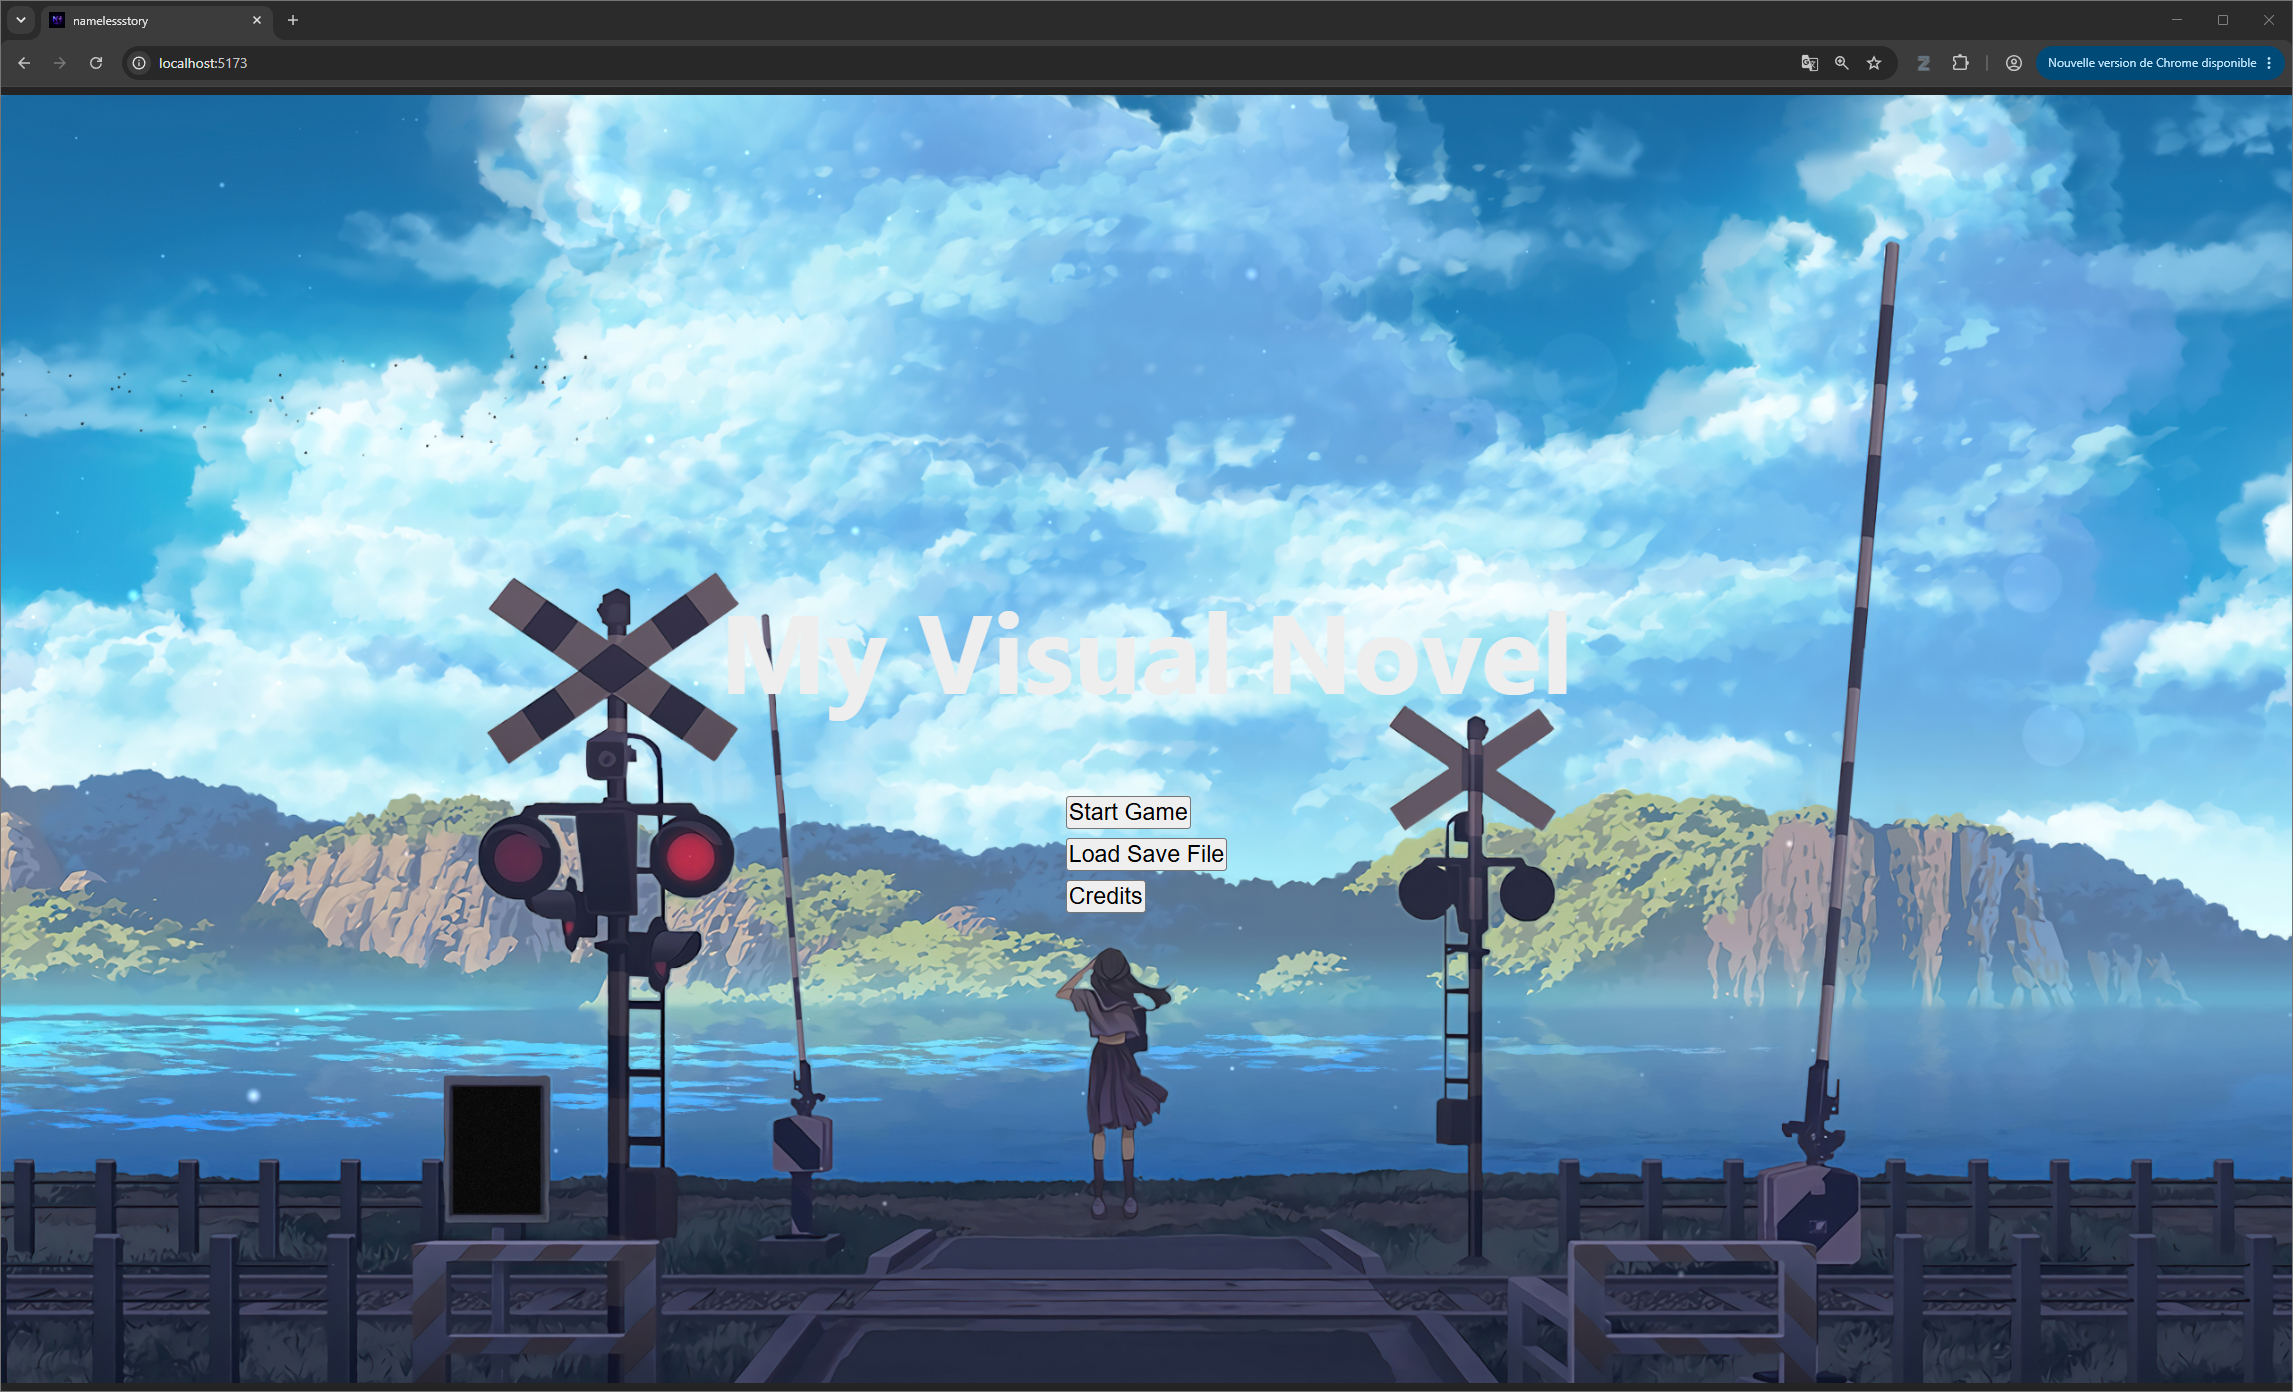
\includegraphics[width=\textwidth]{img/NamelessStory_V1_home.png}
        \caption{Title screen}
    \end{subfigure}
    \hfill
    \begin{subfigure}[b]{0.47\textwidth}
        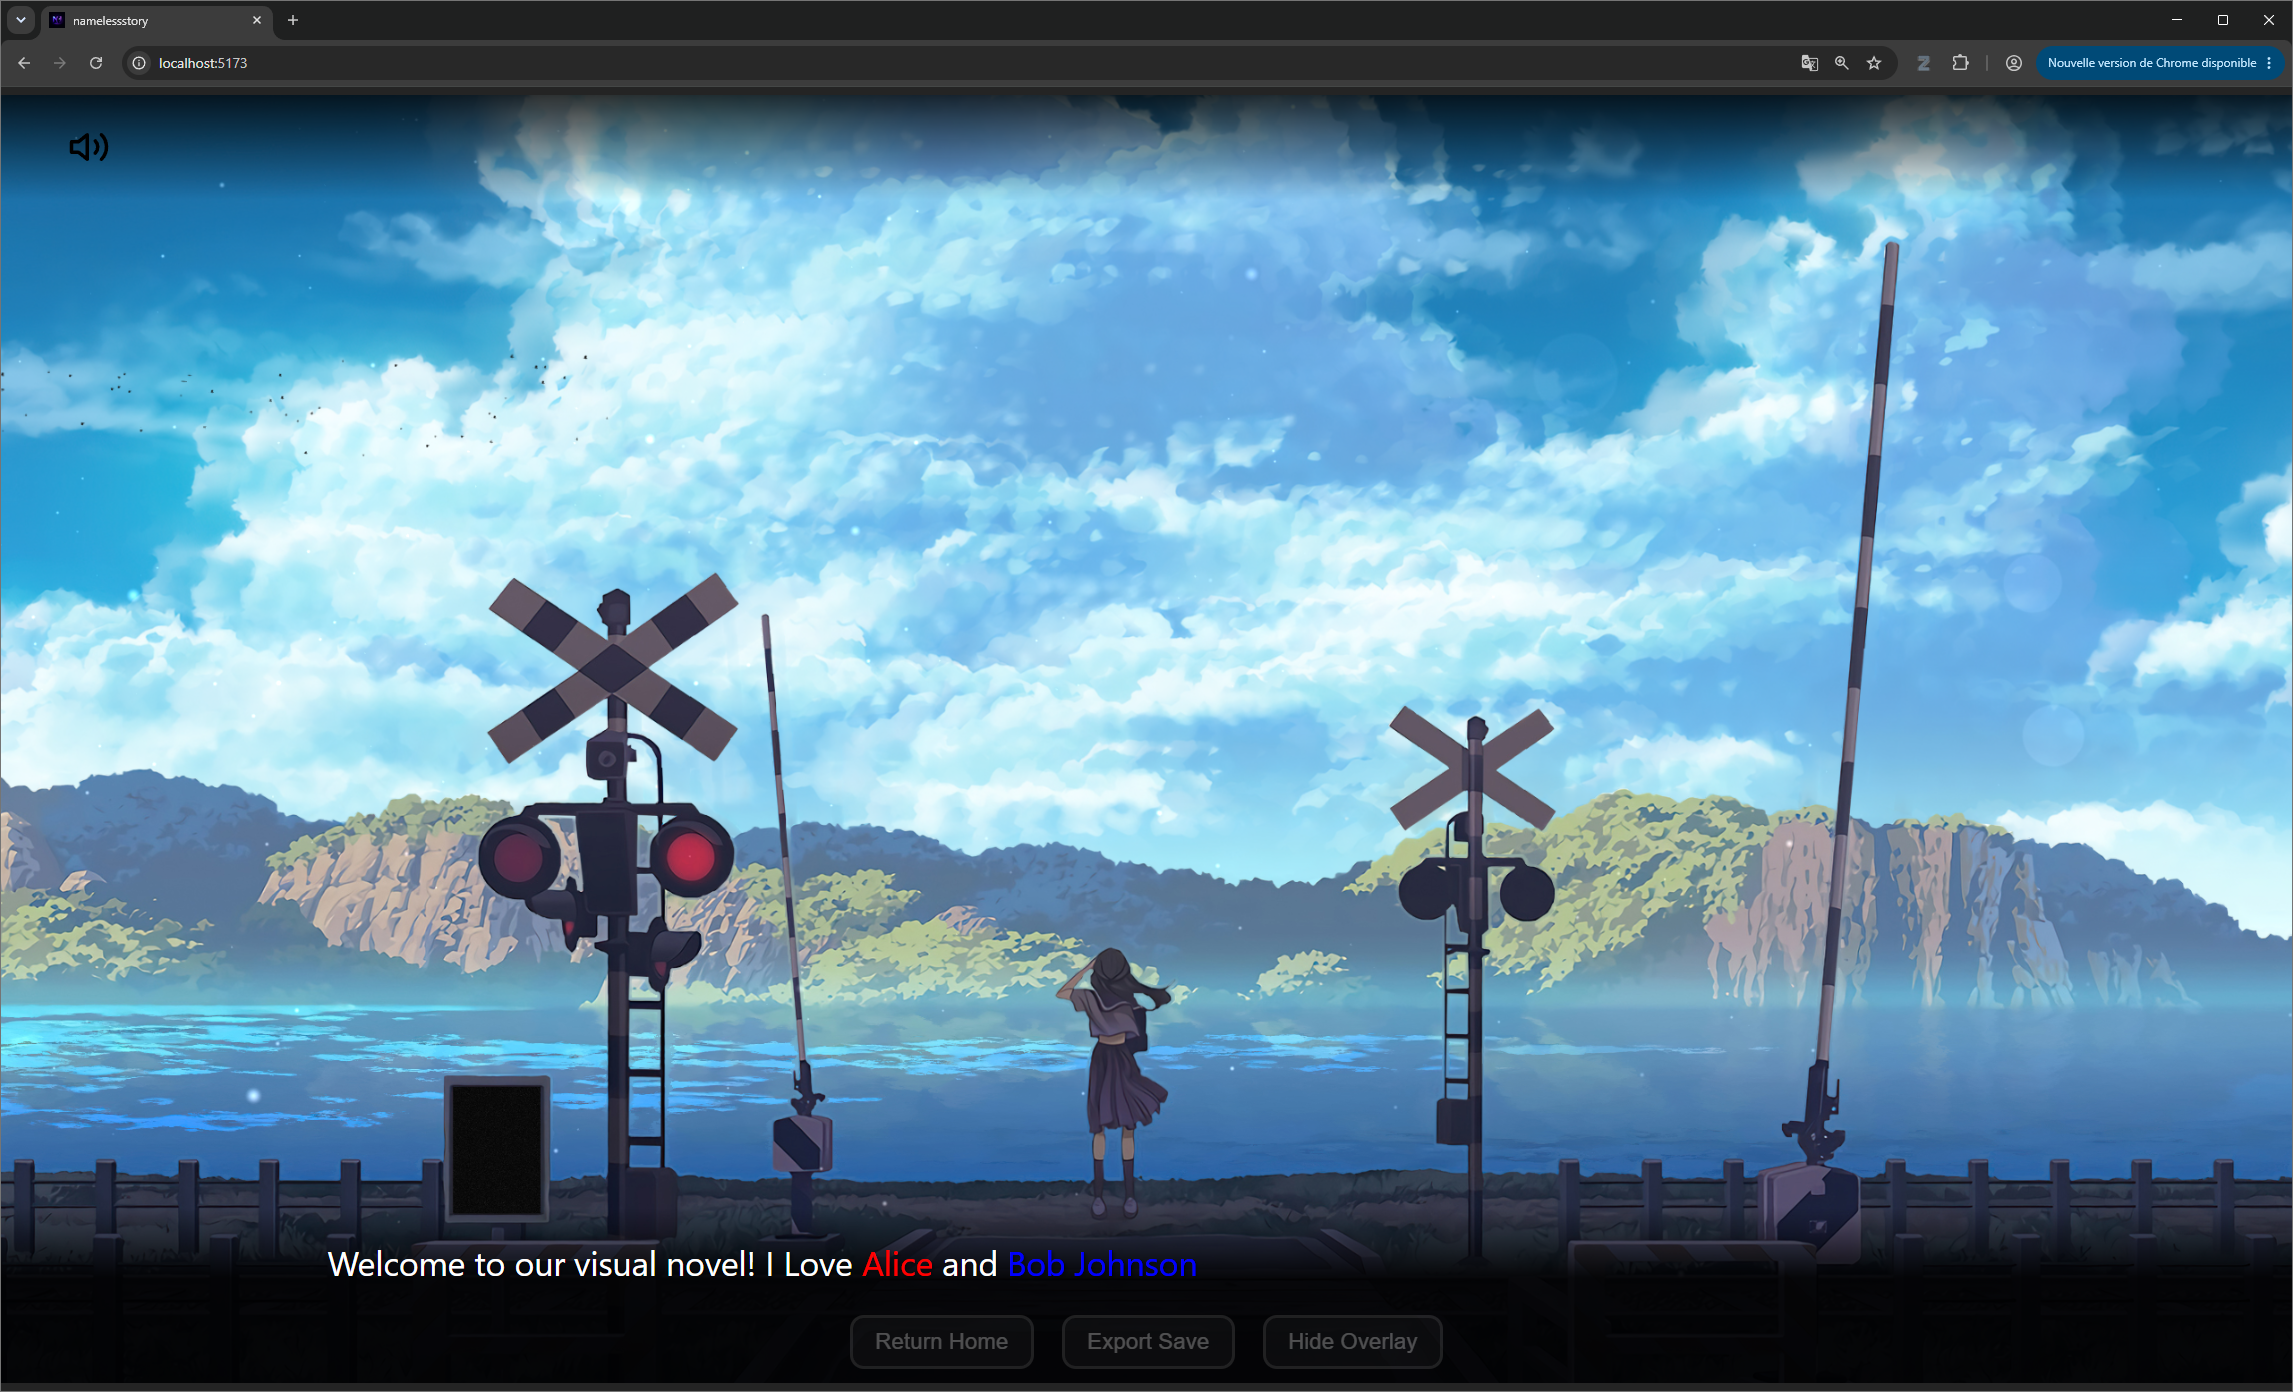
\includegraphics[width=\textwidth]{img/NamelessStory_V1_text.png}
        \caption{Dialogue display}
    \end{subfigure}
    \caption{\nsits at the end of the first iteration (Author 2026)}
    \label{fig:NamelessStoryV1}
\end{figure}

\clearpage


\subsubsubsection{Check}

At the end of this iteration, the core mechanics were functional and verifiable in the browser using a test \gls{json} file. Valid cases were tested manually: dialogue progression on click, navigation to another scene, display of choices, and option selection. Error scenarios were also intentionally constructed (\glsit{negativetesting}), notably by supplying structurally incomplete \gls{json} files, in order to check the engine's behaviour when faced with unexpected data.

These tests revealed that the engine exhibited undefined behaviour when faced with missing or erroneous data, without returning any actionable information to the author: no error message, no way to know what to fix.

Having focused mainly on functionality, the styling was still lacking. What mattered most to me at this stage of the project was having elements displayed on screen, not necessarily that they looked good.


\subsubsubsection{Act}

With a functional baseline in place, two options were open to me going forward: address the error-message problem or optimise the engine's performance. Not yet having the necessary knowledge of robustness and validation, I chose to focus on optimisation work, to ensure the engine avoided unnecessary recomputation and made efficient use of browser resources.

\clearpage


\subsubsection{Second Iteration: Optimisation}

\subsubsubsection{Plan}

The objective of this iteration was to improve the performance and maintainability of the code produced during the first iteration. In \gls{reactjs}, every state update on a parent component triggers a new \gls{rendu} of the entire tree of child components. In a \gls{vn} engine, where the global state changes with every line of dialogue, this behaviour can cause unnecessary recomputation of components whose data has not changed. A second focus concerned save handling: the operation of serialising the current state via \texttt{JSON.stringify()} was running on the browser's main thread. This is not a problem as long as the object to serialise stays modest in size. However, as the state grows richer (game variables, dialogue history, progress data), this operation can become expensive and block the interface for the duration of its execution. To anticipate this limitation, the decision was made to delegate this operation to a \gls{webworker}.


\subsubsubsection{Do}

\Gls{rendu} optimisation was applied across all of the engine's components. Each component was memoised via \texttt{React.memo} (see Section \ref{sec:optim_react}), which allows \gls{reactjs} to short-circuit a component's \gls{rendu} if its \texttt{props} have not changed since the previous \gls{rendu}. For expensive computations performed inside components, the \texttt{useMemo} \glsit{hook} was used to cache results between \glspl{rendu}. References (\texttt{useRef}) also replaced some React state where a value needed to persist without triggering a \glslink{rendu}{re-render}. The \texttt{Typewriter} component in particular underwent significant refactoring: \glslink{snaphtml}{HTML snapshots} and the delays between characters are now precomputed in a single pass before the animation starts, avoiding any recomputation while typing.

Code listing \ref{lst:typewriter} illustrates the \texttt{Typewriter} component's optimisation strategy. Before the animation starts, \texttt{precomputeSteps} computes, in a single pass, all the \glslink{snaphtml}{HTML snapshots} and the delays associated with each character. These snapshots are then converted into React nodes via a second \texttt{useMemo}, whose dependencies are kept strictly separate from the first. During the animation, the tick \texttt{useEffect} is limited to reading \texttt{nodeSnapshots[currentStep]} and scheduling the next call via \texttt{setTimeout} with the precomputed delay \texttt{delays[currentStep]}: no computation is performed on each keystroke.

\begin{listing}[H]
\begin{minted}{ts}
// One-time precomputation: O(n) before the animation
const precomputed = useMemo(
    () => TypewriterUtils.precomputeSteps(tokens, speed),
    [tokens, speed]
);

// Convert HTML snapshots into React nodes (once only)
const nodeSnapshots: ReactNode[] = useMemo(
    () => precomputed.htmlSnapshots.map(htmlToReactNode),
    [precomputed]
);

// Progression: direct index lookup | O(1) per tick
useEffect(() => {
    if (currentStep >= totalSteps) {
        if (!completedRef.current) {
            completedRef.current = true;
            onComplete?.();
        }
        return;
    }
    const delay: number = precomputed.delays[currentStep] ?? speed;
    const timeout: number = setTimeout(
        () => setCurrentStep((prev) => prev + 1),
        delay
    );
    return () => clearTimeout(timeout);
}, [currentStep, totalSteps, precomputed, speed, onComplete]);
\end{minted}
\caption{Precomputation of HTML snapshots and delays in the \textit{Typewriter} component (Author 2026)}
\label{lst:typewriter}
\end{listing}

At the same time, text formatting was reworked for security and robustness reasons. The React \texttt{dangerouslySetInnerHTML} property, which allowed \acrshort{html} to be injected directly into the \acrshort{dom}, was replaced by a pair of dedicated functions: \texttt{escapeHtml}, which neutralises special characters before any processing, and \texttt{htmlToReactNode}, which converts the resulting string into native React nodes. This approach removes the risk of malicious content injection while keeping the flexibility of custom markup. To preserve this tag customisation within the text, a \gls{markdown}-inspired \gls{parseur} was put in place.

For saving, a dedicated \gls{webworker} (\texttt{saveWorker}) was set up. The main thread passes the current state to the \gls{webworker} by exchanging messages; the worker runs \texttt{JSON.stringify()} on its own execution thread, then returns the serialised string to the main thread, as illustrated in Figure \ref{fig:webworker-architecture}. This communication is entirely asynchronous: the user interface remains responsive for the entire duration of the operation, regardless of the size of the object being serialised.

\begin{figure}[H]
    \centering
    \begin{tikzpicture}[
    every node/.style = {font=\small, align=center},
    % Internal boxes
    box/.style = {
        rectangle, rounded corners=3pt,
        draw=clrBorder, line width=0.8pt,
        minimum width=3.2cm, minimum height=0.85cm,
        inner sep=5pt
    },
    main/.style  = {box, fill=clrInput},
    work/.style  = {box, fill=clrToken},
    proc/.style  = {box, fill=clrProcess},
    % Arrows
    arrow/.style = {-{Latex[length=5pt,width=4pt]},
                    line width=0.8pt, color=clrArrow},
    asyncarrow/.style = {-{Latex[length=6pt,width=5pt]},
                    line width=1.2pt, color=clrBorder},
    lbl/.style   = {font=\scriptsize\itshape, color=clrNote},
    lblbf/.style = {font=\scriptsize\bfseries, color=clrBorder},
    ]

%% ═══════════════════════════════════════════════════════
%% LEFT COLUMN — Main thread
%% ═══════════════════════════════════════════════════════

% Main thread internal nodes (x = -3.8cm)
\node[main] at (-3.8cm,  2.6cm) (ui)
    {User interface\\
     \footnotesize{rendering (60 FPS)}};

\node[main] at (-3.8cm,  0.5cm) (input)
    {User interactions\\
     \footnotesize{(clicks, input)}};

\node[main] at (-3.8cm, -1.6cm) (dom)
    {DOM update};

% Main thread internal arrows (two-way)
\draw[arrow, -{Latex[length=4pt,width=3.5pt]}]
    ([xshift= 6pt]ui.south)    -- ([xshift= 6pt]input.north);
\draw[arrow, -{Latex[length=4pt,width=3.5pt]}]
    ([xshift=-6pt]input.north) -- ([xshift=-6pt]ui.south);

\draw[arrow, -{Latex[length=4pt,width=3.5pt]}]
    ([xshift= 6pt]input.south) -- ([xshift= 6pt]dom.north);
\draw[arrow, -{Latex[length=4pt,width=3.5pt]}]
    ([xshift=-6pt]dom.north)   -- ([xshift=-6pt]input.south);

% Trigger and confirmation boxes
\node[main, minimum width=2.6cm] at (-0.3cm,  2.6cm) (trigger)
    {Triggering\\a save};

\node[main, minimum width=2cm] at (-0.5cm, -1.4cm) (confirm)
    {Save\\completed \& \\ confirmed};

%% ═══════════════════════════════════════════════════════
%% RIGHT COLUMN — Web Worker
%% ═══════════════════════════════════════════════════════

\node[work] at (5.8cm,  2.6cm) (rawdata)
    {Save data\\
     \footnotesize{(raw object)}};

\node[proc] at (5.8cm,  1.2cm) (stringify)
    {\texttt{JSON.stringify(Object)}};

\node[proc] at (5.8cm,  0.0cm) (jsonstr)
    {Resulting JSON string};

\node[work] at (5.8cm, -1.4cm) (calctime)
    {Computation time\\
     \footnotesize{(non-blocking for the UI)}};

% Web Worker internal arrows
\draw[arrow] (rawdata)   -- (stringify);
\draw[arrow] (stringify) -- (jsonstr);
\draw[arrow] (jsonstr)   -- (calctime);

%% ═══════════════════════════════════════════════════════
%% ASYNCHRONOUS ARROWS between zones
%% ═══════════════════════════════════════════════════════

% Request: trigger -> rawdata
\draw[asyncarrow] ([yshift=-0.4cm]trigger.east)
    -- node[lblbf, below=3pt, text width=1.7cm, xshift=-0.1cm, fill=clrOutput!40, line width=0.6pt, draw=clrOutput, rounded corners=3pt] {async request}
    ([yshift=-0.4cm]rawdata.west);

% Response: calctime -> confirm
\draw[asyncarrow] ([yshift=-0.4cm]calctime.west)
    -- node[lblbf, below=6pt, text width=1.7cm, xshift=0.2cm, fill=clrOutput!40, line width=0.6pt, draw=clrOutput, rounded corners=3pt] {async response}
    ([yshift=-0.4cm]confirm.east);

%% ═══════════════════════════════════════════════════════
%% BOUNDING BOXES
%% ═══════════════════════════════════════════════════════

\begin{scope}[on background layer]
  \node[draw=clrBorder, rounded corners=6pt,
        fill=clrInput!40, line width=1pt,
        fit=(ui)(input)(dom)(trigger)(confirm),
        inner sep=12pt,
        label={[font=\normalsize\bfseries, text=clrBorder]
               above:Main Thread}
       ] (mainbox) {};

  \node[draw=clrBorder, rounded corners=6pt,
        fill=clrToken!40, line width=1pt,
        fit=(rawdata)(stringify)(jsonstr)(calctime),
        inner sep=12pt,
        label={[font=\normalsize\bfseries, text=clrBorder]
               above:Web Worker \normalfont\footnotesize (dedicated to serialisation)}
       ] (workerbox) {};
\end{scope}

    \end{tikzpicture}
    \caption{Main thread/Web Worker separation architecture for saving (Author 2026)}
    \label{fig:webworker-architecture}
\end{figure}


Code listing \ref{lst:saveworker} presents the two components of this architecture. On the secondary-thread side, the \texttt{worker} receives, via \texttt{postMessage}, an object containing the current state and the target cookie's name, runs \texttt{JSON.stringify} on its own execution thread, then returns the serialised string together with the cookie name. This coupling guarantees that the \gls{webworker} retains no data between calls: it receives all the information it needs with each message and can be reused for any save operation with no additional initialisation. On the main-thread side, the \gls{webworker} is instantiated only once, when the component is initialised, via \texttt{useEffect}, and is kept in a \texttt{useRef} reference to avoid repeated instantiation. The \texttt{onmessage} callback receives the result asynchronously and triggers the cookie write without ever having blocked the \gls{rendu} thread.

\begin{listing}[H]
\begin{minted}{ts}
// workers/saveWorkers.ts (secondary thread)
self.addEventListener("message",
    (e: MessageEvent<SaveWorkerMessage>) => {
        const { state, cookieName } = e.data;
        const serialized = JSON.stringify(state);
        (self as unknown as Worker).postMessage(
            { serialized, cookieName } satisfies SaveWorkerResponse
        );
    }
);


// VisualNovel/index.tsx (main thread)
const saveWorkerRef = useRef<Worker | null>(null);

useEffect(() => {
    const worker = new Worker(
        new URL('../../../workers/saveWorker.ts', import.meta.url),
        { type: 'module' }
    );
    worker.addEventListener('message',
        (e: MessageEvent<SaveWorkerResponse>) => {
            saveState(e.data.cookieName, e.data.serialized);
        }
    );
    saveWorkerRef.current = worker;
    return () => {
        worker.terminate();
        saveWorkerRef.current = null;
    };
}, []);
\end{minted}
\caption{Implementation of \texttt{saveWorker}: communication protocol between the main thread and the secondary thread (Author 2026)}
\label{lst:saveworker}
\end{listing}

\clearpage


\subsubsubsection{Check}

After several trial runs of the engine, the features implemented during the first iteration were checked and found to be unaffected by the changes made.

To assess the impact of the optimisations on rendering performance, five identical test sessions were recorded using \gls{reactprofiler}, on the version prior to the optimisations (\textit{commit}\footnote{\textbf{Commit}: in \gls{git}, a record of a set of changes made to the source code at a given point in time, identified by a unique fingerprint (hash) allowing it to be reverted to or referenced precisely. \parencite{noauthor_git_nodate}} \texttt{9831b9e}) and on the optimised version. Each session followed the same sequence of interactions on the same test \gls{json} file, in the same browser.

\clearpage

Tables \ref{tab:profiling_before} and \ref{tab:profiling_after} present the four metrics recorded: the total number of \glspl{rendu}, the average duration per \gls{rendu}, the maximum duration observed, and the cumulative duration of all \glspl{rendu} in the session.

\begin{table}[H]
    \centering
    \caption{Performance measurements before optimisation (five sessions)}
    \renewcommand{\arraystretch}{1.5}
    \begin{tabular}{p{0.8cm} p{2.5cm} p{3cm} p{3cm} p{3cm}}
        \hline
        \textbf{No.} & \textbf{Renders} & \textbf{Avg. duration (ms)} & \textbf{Max. duration (ms)} & \textbf{Total duration (ms)} \\
        \hline
        1 & 688 & 0.165 & 2.90 & 113.70 \\
        2 & 689 & 0.166 & 2.90 & 114.50 \\
        3 & 689 & 0.161 & 3.10 & 111.00 \\
        4 & 688 & 0.168 & 3.10 & 115.70 \\
        5 & 688 & 0.163 & 3.00 & 112.10 \\
        \hline
        \textbf{*} & \textbf{688} & \textbf{0.165} & \textbf{3.00} & \textbf{113.70} \\
        \hline
    \end{tabular}
    \par\smallskip{\footnotesize * Median of the five sessions}
    \label{tab:profiling_before}
\end{table}

\begin{table}[H]
    \centering
    \caption{Performance measurements after optimisation (five sessions)}
    \renewcommand{\arraystretch}{1.5}
    \begin{tabular}{p{0.8cm} p{2.5cm} p{3cm} p{3cm} p{3cm}}
        \hline
        \textbf{No.} & \textbf{Renders} & \textbf{Avg. duration (ms)} & \textbf{Max. duration (ms)} & \textbf{Total duration (ms)} \\
        \hline
        1 & 476 & 0.335 & 19.90 & 159.50 \\
        2 & 492 & 0.320 & 18.30 & 157.60 \\
        3 & 492 & 0.327 & 18.40 & 161.10 \\
        4 & 492 & 0.321 & 18.30 & 158.00 \\
        5 & 493 & 0.321 & 18.20 & 158.30 \\
        \hline
        \textbf{*} & \textbf{492} & \textbf{0.321} & \textbf{18.30} & \textbf{158.30} \\
        \hline
    \end{tabular}
    \par\smallskip{\footnotesize * Median of the five sessions}
    \label{tab:profiling_after}
\end{table}

\clearpage

Figures \ref{fig:profiling_renders} and \ref{fig:profiling_maxdur} illustrate, respectively, the change in the number of \glspl{rendu} and in the maximum duration between the two versions.

\begin{figure}[H]
    \centering
    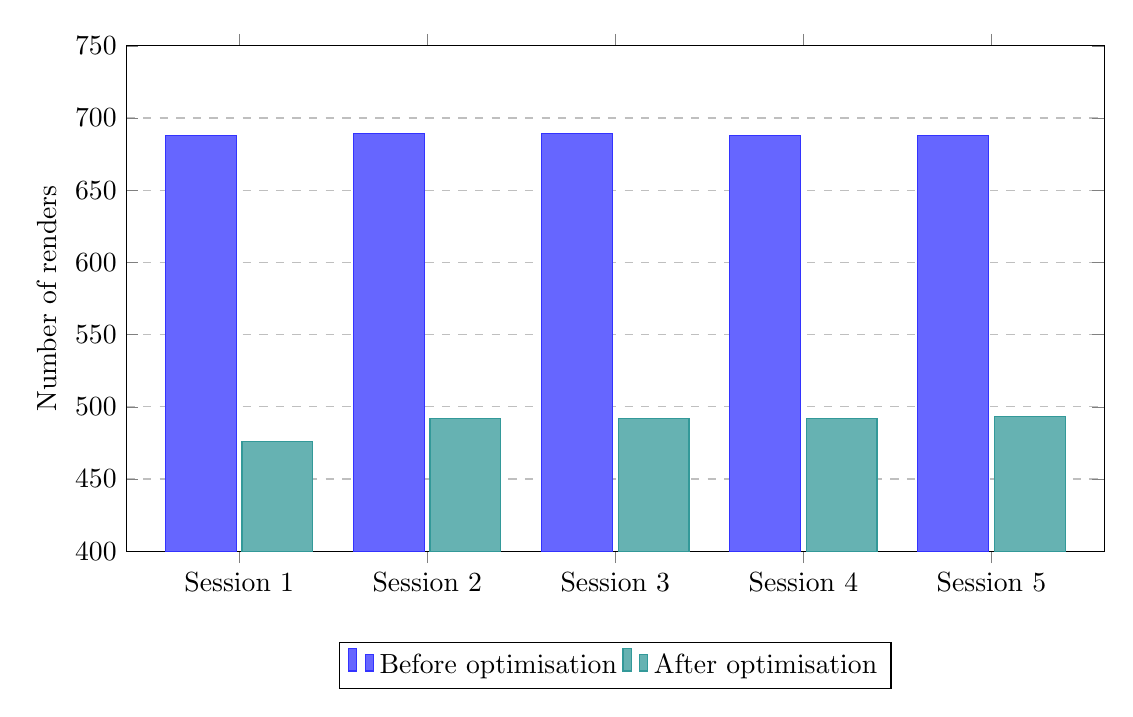
\begin{tikzpicture}
        \begin{axis}[
            ybar,
            bar width=0.9cm,
            width=14cm,
            height=8cm,
            ymin=400,
            ymax=750,
            ylabel={Number of renders},
            xtick=data,
            xticklabels={Session 1, Session 2, Session 3, Session 4, Session 5},
            legend style={at={(0.5,-0.18)}, anchor=north, legend columns=2},
            ymajorgrids=true,
            grid style=dashed,
            enlarge x limits=0.15,
        ]
        \addplot[fill=blue!60, draw=blue!80]
            coordinates {(1,688) (2,689) (3,689) (4,688) (5,688)};
        \addplot[fill=teal!60, draw=teal!80]
            coordinates {(1,476) (2,492) (3,492) (4,492) (5,493)};
        \legend{Before optimisation, After optimisation}
        \end{axis}
    \end{tikzpicture}
    \caption{Number of renders per session before and after optimisation (\textit{commit} \texttt{9831b9e}) measured via React DevTools Profiler (Author 2026)}
    \label{fig:profiling_renders}
\end{figure}

\begin{figure}[H]
    \centering
    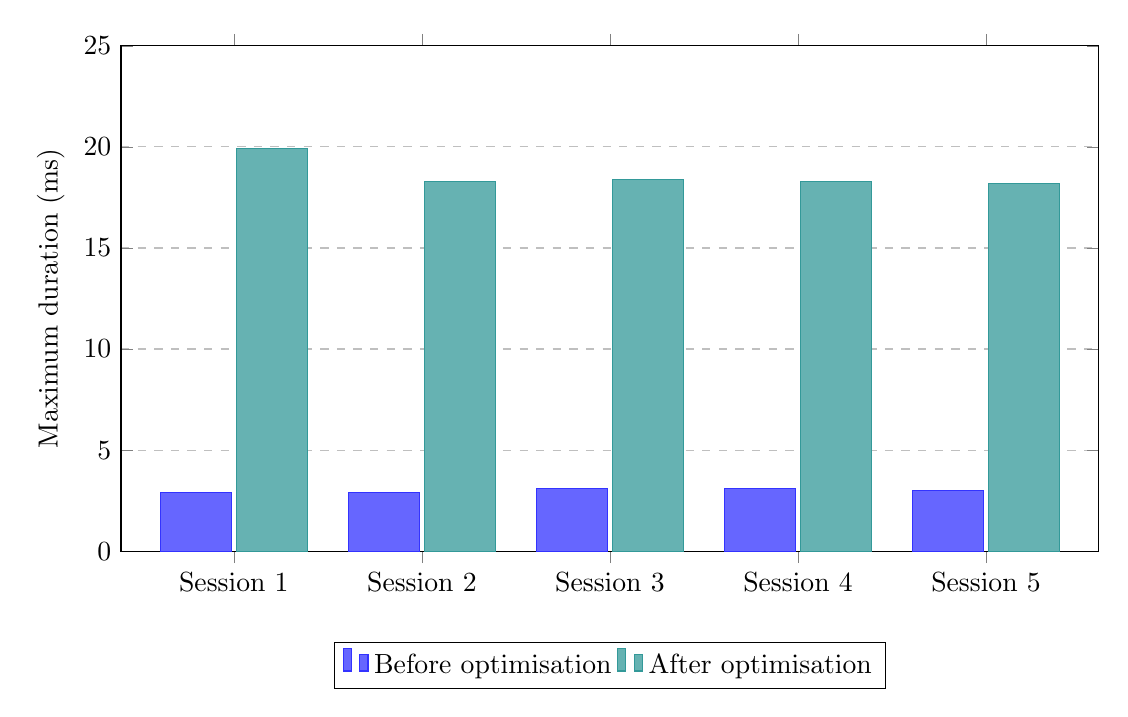
\begin{tikzpicture}
        \begin{axis}[
            ybar,
            bar width=0.9cm,
            width=14cm,
            height=8cm,
            ymin=0,
            ymax=25,
            ylabel={Maximum duration (ms)},
            xtick=data,
            xticklabels={Session 1, Session 2, Session 3, Session 4, Session 5},
            legend style={at={(0.5,-0.18)}, anchor=north, legend columns=2},
            ymajorgrids=true,
            grid style=dashed,
            enlarge x limits=0.15,
        ]
        \addplot[fill=blue!60, draw=blue!80]
            coordinates {(1,2.9) (2,2.9) (3,3.1) (4,3.1) (5,3.0)};
        \addplot[fill=teal!60, draw=teal!80]
            coordinates {(1,19.9) (2,18.3) (3,18.4) (4,18.3) (5,18.2)};
        \legend{Before optimisation, After optimisation}
        \end{axis}
    \end{tikzpicture}
    \caption{Maximum render duration per session before and after optimisation (\textit{commit} \texttt{9831b9e}) measured via React DevTools Profiler (Author 2026)}
    \label{fig:profiling_maxdur}
\end{figure}

\clearpage

The measurements reveal a nuanced result. The number of \glspl{rendu} decreased by 28.5\% (688 → 492), confirming the effect of \texttt{React.memo}: unnecessary \glslink{rendu}{re-renders} were eliminated. On the other hand, the average duration per \gls{rendu} increased (0.165ms → 0.321ms), and the peak maximum rose from 3ms to 18.3ms. This behaviour is consistent with the precomputation strategy adopted by the \texttt{Typewriter} component: the computational cost is concentrated on the initial \gls{rendu} rather than spread across each displayed character. For comparable overall performance, the optimised version therefore places a lighter load on the browser's main thread over the course of a session.


\subsubsubsection{Act}

With the optimisations made during this iteration having met their main objective, the next area of work had already been identified since the first iteration: error handling and data validation. With the engine now performant, it was time to ensure it was also robust when faced with invalid or incomplete \gls{json} files. The third iteration was therefore dedicated to researching and implementing a \gls{schema} validation system.


\subsubsection{Third Iteration: Security and Robustness}

\subsubsubsection{Plan}

The objective of this iteration was to address the main limitation identified during the previous iterations: the absence of formal validation of the \acrshort{json} files supplied by the author. Without a verification mechanism, a syntactically invalid file, or one that did not conform to the expected \gls{schema}, could put the engine into an indeterminate state, with no actionable feedback for the author. Integrating the \gls{zod} \gls{librairie}, presented in Section \ref{sec:zod}, was the response to this gap.

Discovering \gls{zod} was not the result of a targeted search, but of a chance encounter on GitHub, where the \gls{librairie} appeared frequently in \gls{ts} projects dealing with \gls{schema} validation. Before adopting it, two alternatives were evaluated: TypeBox\footnote{\textbf{TypeBox}: \gls{json}-based \gls{ts} \gls{schema} validation \gls{librairie}, developed by Haydn Paterson \parencite{noauthor_typebox_nodate}} and ArkType\footnote{\textbf{ArkType}: validation and type-inference \gls{librairie} for \gls{ts}, focused on performance and a \gls{syntaxe} inspired by the language's native notation \parencite{noauthor_arktype_nodate}}. TypeBox offers an approach similar to \gls{zod}, while ArkType relies on a noticeably different \gls{syntaxe}, which proved less immediate to pick up. The choice ultimately fell on \gls{zod} for the conciseness and readability of its \gls{syntaxe}, an important criterion when it comes to keeping the code accessible to the project's potential contributors.

\clearpage

This iteration also made it possible to implement several \textit{Can} features identified in Table \ref{tab:objectifs_moscow}, which available time had not allowed integrating during the previous iterations: displaying character \glsplit{sprite} with dynamic positioning, transitions between scenes and dialogues, font management via \acrshort{css} variables, and support for a dynamic \glsit{placeholder} for input fields.


\subsubsubsection{Do}

The integration of \gls{zod} was built around two distinct validation \glspl{schema}. The first, \texttt{storySchema}, describes the expected structure of the scenario's \acrshort{json} file: node types, presence of required fields, allowed values for enumerated properties. The second, \texttt{saveSchema}, covers the structure of save files, in order to detect and reject any corrupted or manually modified file before it is passed to the engine. In case of a discrepancy from the defined \gls{schema} (missing field, incorrect type, invalid structure), \gls{zod} returns an explicit error message precisely indicating the location and nature of the problem, which constitutes a deterministic error-detection mechanism and direct feedback for the author.

Code listing \ref{lst:storyschema} presents an excerpt of \texttt{VNStorySchema}. Validation operates on two levels. The first is declarative: each field of the \gls{json} file is explicitly typed via \gls{zod} primitives (\texttt{z.string()}, \texttt{z.number().positive()}, \texttt{z.enum([...])}), which makes it possible to catch at runtime any missing field, incorrect type, or value outside the allowed options. The second level, implemented via \texttt{superRefine}, performs cross-field semantic validation that cannot be expressed with types alone: it checks that the scene referenced by \texttt{startingScene} does exist in the \texttt{story} block, and that every navigation target (the \texttt{next} fields of dialogues and options) points to a declared scene. In case of a discrepancy, \texttt{ctx.addIssue} produces an error message including the exact path of the offending field, as illustrated in Figure \ref{fig:zod_erreurs}.

\begin{listing}[H]
\begin{minted}{ts}
const DialogueSchema = z.object({
    next: z.string().optional(),
    options: z.array(OptionSchema).optional(),
});

export const VNStorySchema = z.object({
    settings: SettingsSchema,
    story: z.record(z.string(), SceneTypeSchema),
}).superRefine((data, ctx) => {
    if (!data.story[data.settings.startingScene]) {
        ctx.addIssue({
            code: "custom",
            message: `"${data.settings.startingScene}" does not exist in Story`,
            path: ["settings", "startingScene"],
        });
    }
    for (const [sceneId, scene] of Object.entries(data.story)) {
        scene.dialogues.forEach((dialogue, i) => {
            const refs = [
                ...(dialogue.next ? [{val: dialogue.next, path: ["next"]}] : []),
                ...(dialogue.options ?? []).map(o => ({val: o.next, path: ["options"]})),
            ];
            refs.forEach(({val, path}) => {
                const target = val.split(":")[0];
                if (!data.story[target] && target !== END_STORY_TOKEN) {
                    ctx.addIssue({
                        code: "custom",
                        message: `Scene "${target}" does not exist`,
                        path: ["story", sceneId, "dialogues", i, ...path],
                    });
                }
            });
        });
    }
});
\end{minted}
\caption{Excerpt of \texttt{VNStorySchema}: declarative validation and semantic verification of navigation references (Author 2026)}
\label{lst:storyschema}
\end{listing}

\clearpage

To cover error cases systematically, dedicated test files were added to the repository in a \texttt{tests/} folder. These files intentionally represent invalid scenarios: \acrshort{json} with broken \gls{syntaxe} (missing comma, unclosed quotation mark), files with missing required fields, and files with incorrect-type values. These files are excluded from the production \glsit{build} via a dedicated \gls{vite} \glsit{plugin}.


\subsubsubsection{Check}

The \glslink{negativetesting}{negative tests} carried out at the end of this iteration covered all of the cases described above. In each case, \gls{zod} returned an explicit error message and the engine remained in a stable state, confirming the expected behaviour, as illustrated in Figure \ref{fig:zod_erreurs}.

\begin{figure}[H]
    \centering
    \begin{subfigure}[b]{0.47\textwidth}
        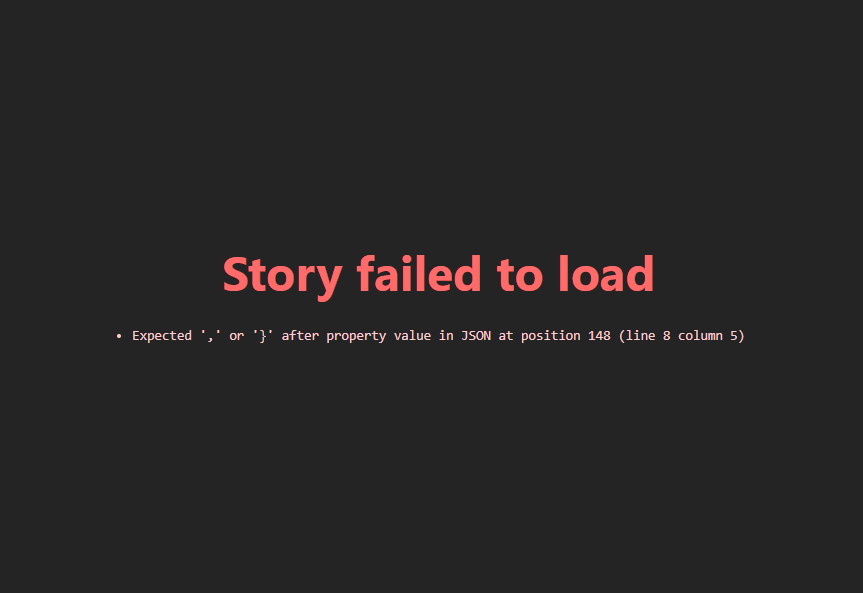
\includegraphics[height=4.85cm]{img/zod_invalid_syntax_1.png}
        \caption{JSON syntax error}
    \end{subfigure}
    \hfill
    \begin{subfigure}[b]{0.47\textwidth}
        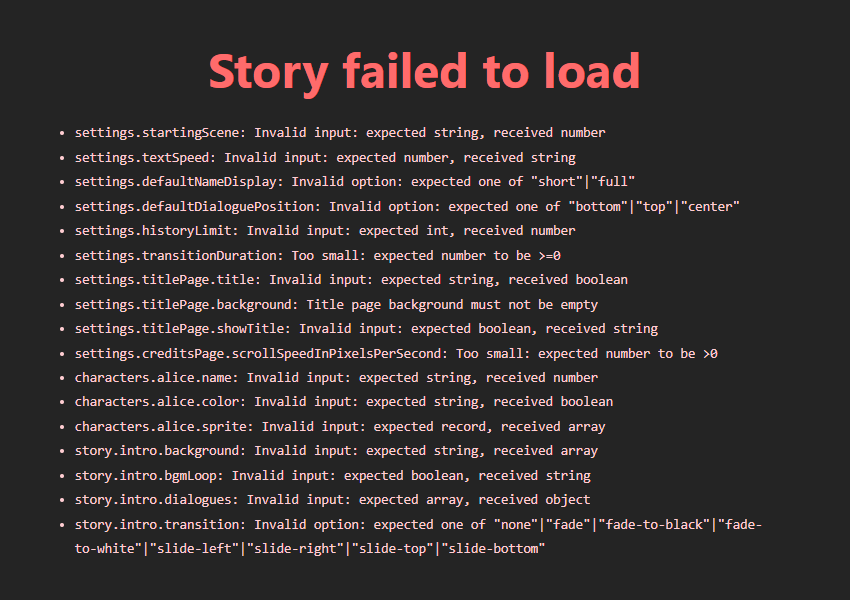
\includegraphics[height=4.85cm]{img/zod_missing_field_1.png}
        \caption{Missing required fields}
    \end{subfigure}
    \caption{Error messages returned by Zod when validating the JSON file (Author 2026)}
    \label{fig:zod_erreurs}
\end{figure}

Save file validation was also tested by supplying manually modified files, which were correctly rejected with an error message surfacing all the way up to the title screen.

\clearpage

Figure \ref{fig:NamelessStoryFinal} presents the state of the engine at the end of these three iterations. The remark made in footnote \ref{fn:zoom175} about browser zoom also applies to these screenshots. The \gls{json} file used for this screenshot differs from the one used in the first iteration: rather than a short story, it is a demo (\textit{"The Feature Tour"}) running through all the features implemented in the engine.

\begin{figure}[H]
    \centering
    \begin{subfigure}[b]{0.47\textwidth}
        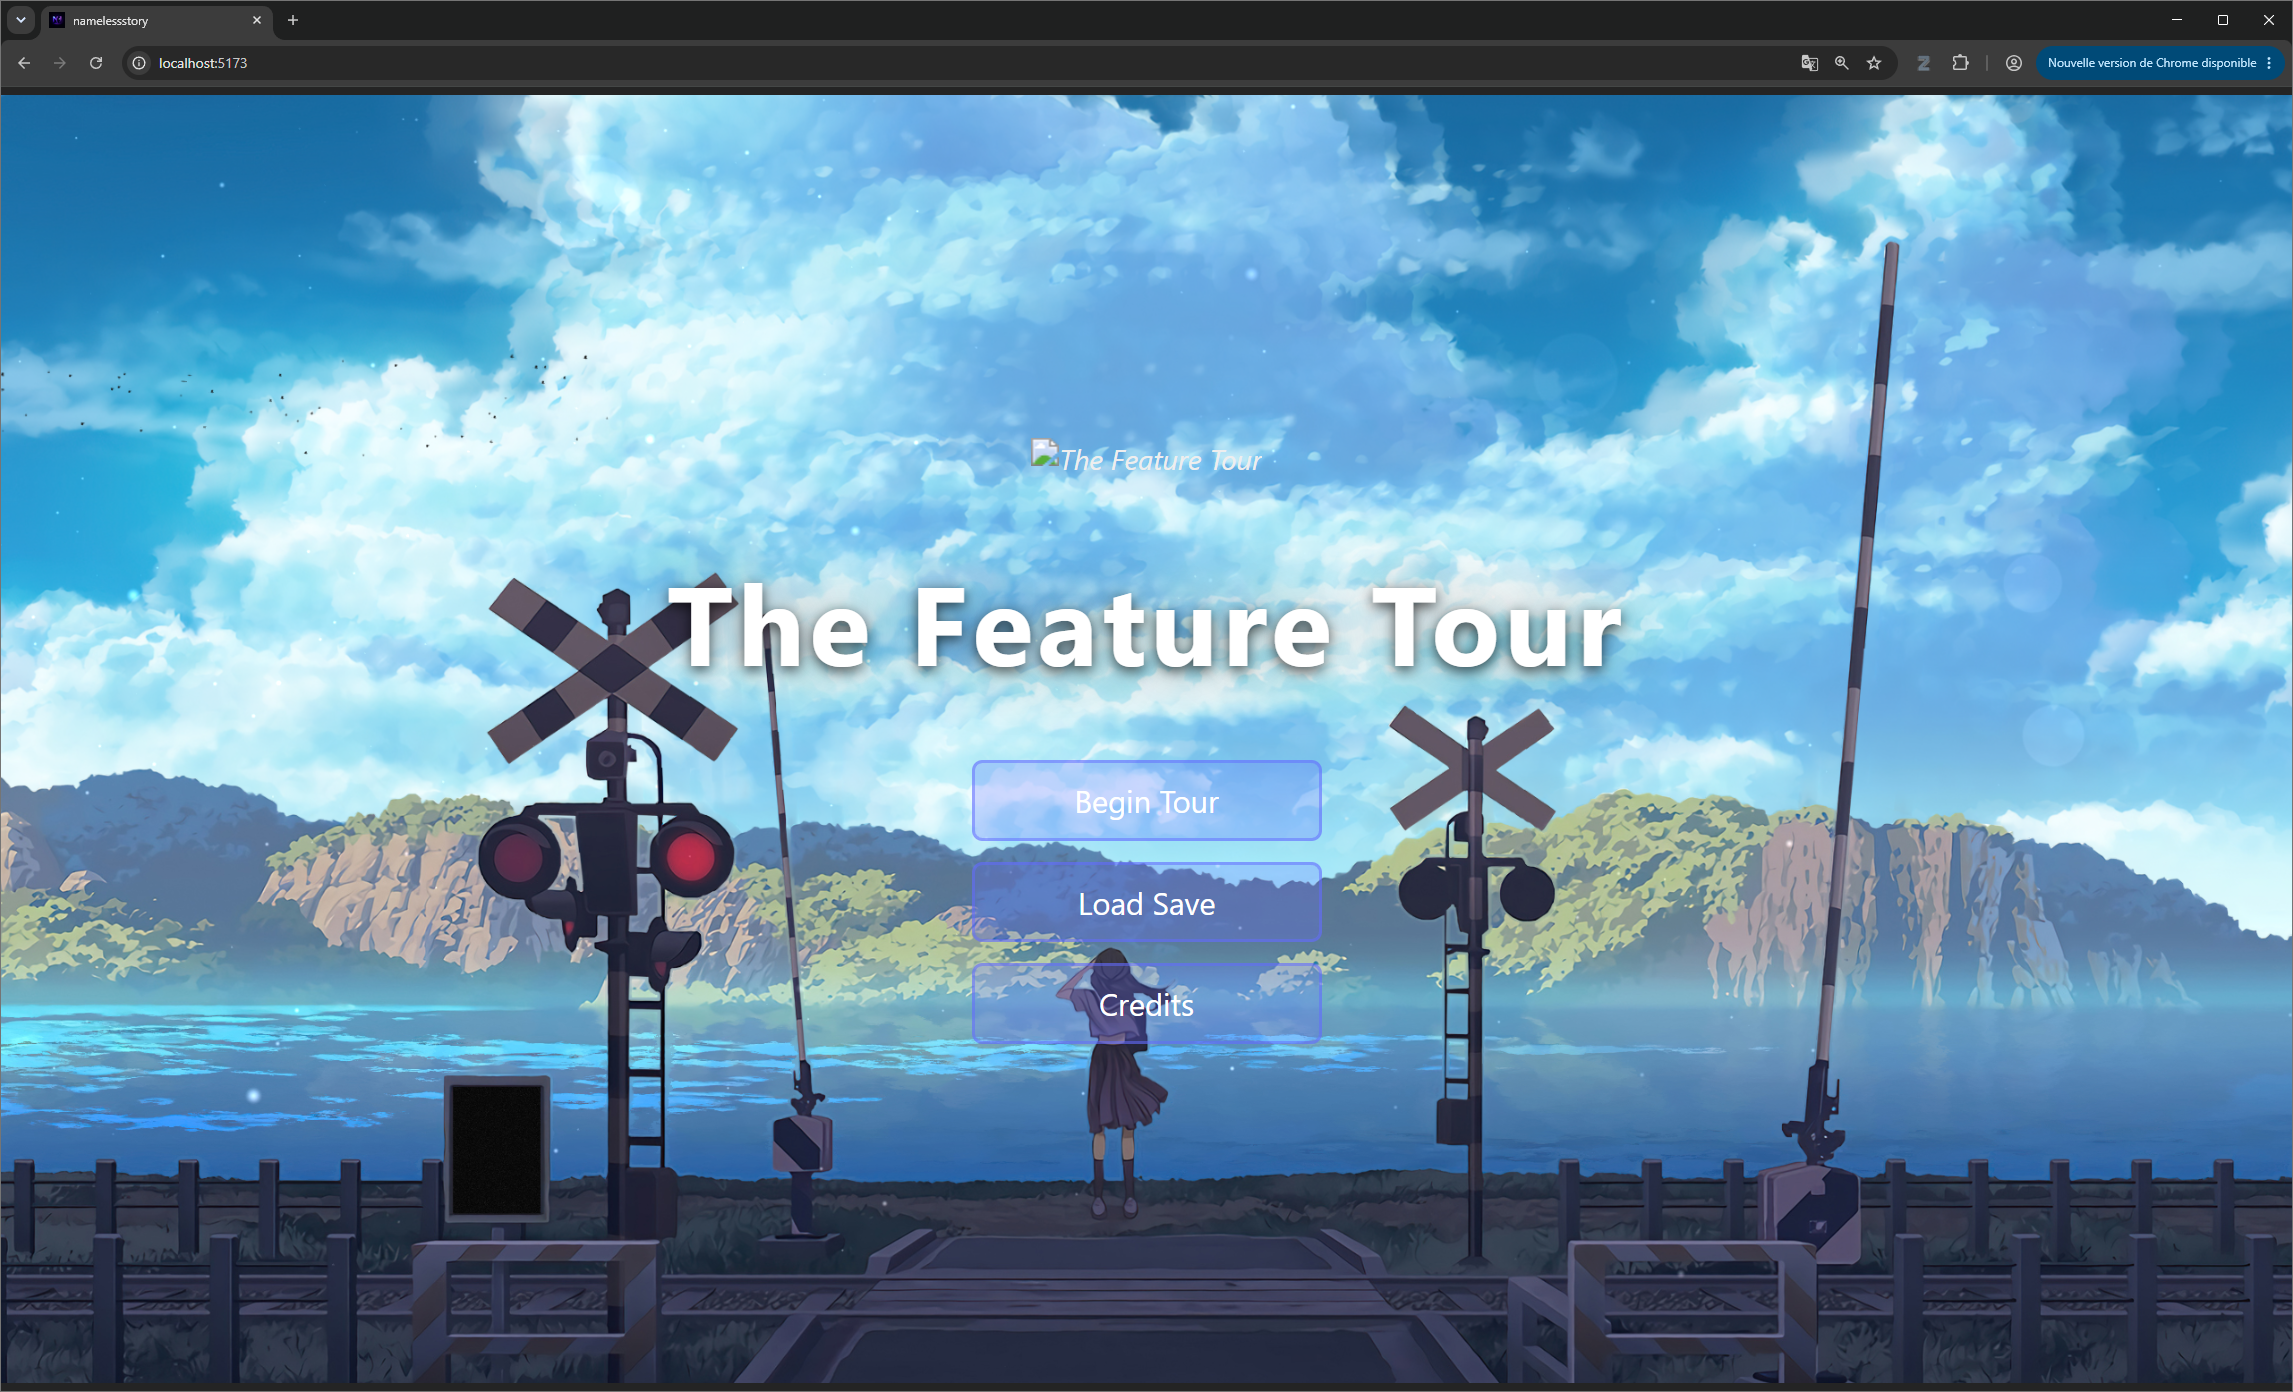
\includegraphics[width=\textwidth]{img/NamelessStory_final_home.png}
        \caption{Title screen}
    \end{subfigure}
    \hfill
    \begin{subfigure}[b]{0.47\textwidth}
        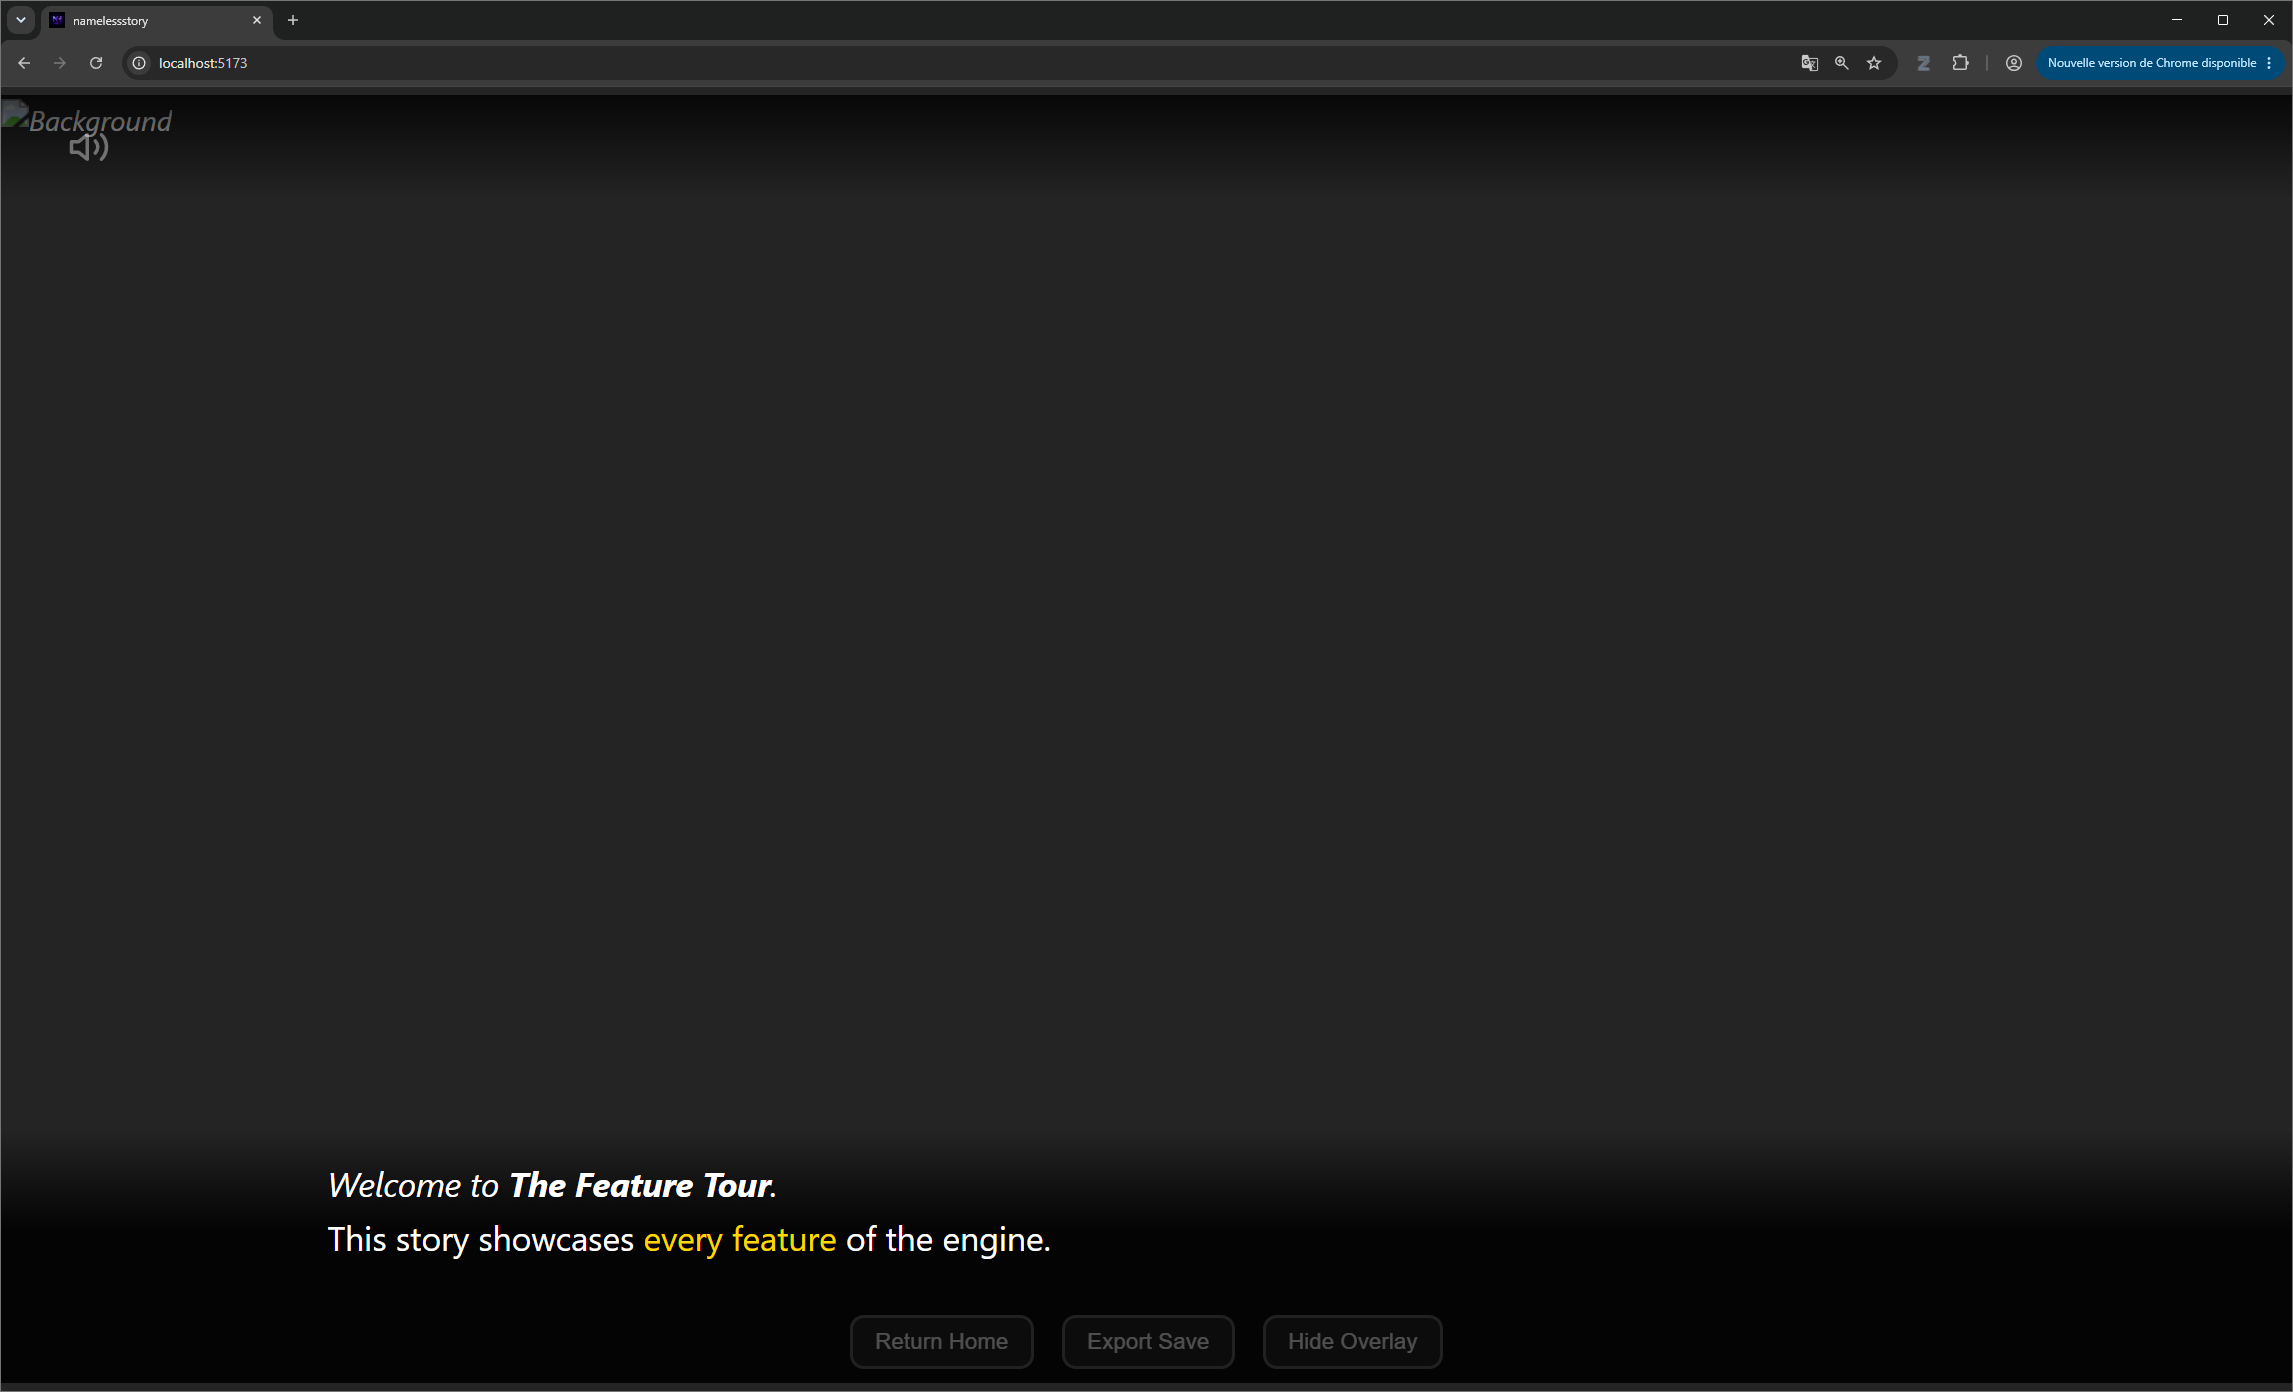
\includegraphics[width=\textwidth]{img/NamelessStory_final_text.png}
        \caption{Dialogue display}
    \end{subfigure}
    \caption{\nsits at the end of the third iteration (Author 2026)}
    \label{fig:NamelessStoryFinal}
\end{figure}


\subsubsubsection{Act}

At the end of this iteration, all of the \textit{Must} and \textit{Should} objectives defined in Table \ref{tab:objectifs_moscow} had been met. Several \textit{Can} features were also integrated. The remaining out-of-scope features (notably a built-in scenario editor and advanced handling of complex narrative branching) are identified as future development directions in Chapter \ref{chap:resultats}.
